%%%%%%%%%%%%%%%%%%%%%%%%%%%%%%%%%%%%%%%
% Wenneker Resume/CV
% LaTeX Template
% Version 1.1 (19/6/2016)
%
% This template has been downloaded from:
% http://www.LaTeXTemplates.com
%
% Original author:
% Frits Wenneker (http://www.howtotex.com) with extensive modifications by 
% Vel (vel@LaTeXTemplates.com)
%
% License:
% CC BY-NC-SA 3.0 (http://creativecommons.org/licenses/by-nc-sa/3.0/
%
%%%%%%%%%%%%%%%%%%%%%%%%%%%%%%%%%%%%%%

%----------------------------------------------------------------------------------------
%	PACKAGES AND OTHER DOCUMENT CONFIGURATIONS
%----------------------------------------------------------------------------------------

\documentclass[a4paper,12pt]{memoir} % Font and paper size

%%%%%%%%%%%%%%%%%%%%%%%%%%%%%%%%%%%%%%%%%
% Wenneker Resume/CV
% Structure Specification File
% Version 1.1 (19/6/2016)
%
% This file has been downloaded from:
% http://www.LaTeXTemplates.com
%
% Original author:
% Frits Wenneker (http://www.howtotex.com) with extensive modifications by 
% Vel (vel@latextemplates.com)
%
% License:
% CC BY-NC-SA 3.0 (http://creativecommons.org/licenses/by-nc-sa/3.0/)
%
%%%%%%%%%%%%%%%%%%%%%%%%%%%%%%%%%%%%%%%%%

%----------------------------------------------------------------------------------------
%	PACKAGES AND OTHER DOCUMENT CONFIGURATIONS
%----------------------------------------------------------------------------------------

\usepackage{XCharter} % Use the Bitstream Charter font
\usepackage[utf8]{inputenc} % Required for inputting international characters
\usepackage[T1]{fontenc} % Output font encoding for international characters

\usepackage[top=1cm,left=1cm,right=1cm,bottom=1cm]{geometry} % Modify margins

\usepackage{graphicx} % Required for figures

\usepackage{flowfram} % Required for the multi-column layout

\usepackage{url} % URLs

\usepackage[usenames,dvipsnames]{xcolor} % Required for custom colours

\usepackage{tikz} % Required for the horizontal rule

\usepackage{enumitem} % Required for modifying lists
\setlist{noitemsep,nolistsep} % Remove spacing within and around lists

\setlength{\columnsep}{\baselineskip} % Set the spacing between columns

% Define the left frame (sidebar)
\newflowframe{0.3\textwidth}{\textheight}{0pt}{0pt}[left]
\newlength{\LeftMainSep}
\setlength{\LeftMainSep}{0.3\textwidth}
\addtolength{\LeftMainSep}{0.5\columnsep}
 
% Small static frame for the vertical line
\newstaticframe{1.5pt}{\textheight}{\LeftMainSep}{0pt}
 
% Content of the static frame with the vertical line
\begin{staticcontents}{1}
\hfill
\tikz{\draw[loosely dotted,color=RoyalBlue,line width=1.5pt,yshift=0](0,0) -- (0,\textheight);}
\hfill\mbox{}
\end{staticcontents}
 
% Define the right frame (main body)
\addtolength{\LeftMainSep}{1.5pt}
\addtolength{\LeftMainSep}{1\columnsep}
\newflowframe{0.6\textwidth}{\textheight}{\LeftMainSep}{0pt}[main01]

\pagestyle{empty} % Disable all page numbering

\setlength{\parindent}{0pt} % Stop paragraph indentation

%----------------------------------------------------------------------------------------
%	NEW COMMANDS
%----------------------------------------------------------------------------------------

\newcommand{\userinformation}[1]{\renewcommand{\userinformation}{#1}} % Define a new command for the CV user's information that goes into the left column

\newcommand{\cvheading}[1]{{\Huge\bfseries\color{RoyalBlue} #1} \par\vspace{.6\baselineskip}} % New command for the CV heading
\newcommand{\cvsubheading}[1]{{\Large\bfseries #1} \bigbreak} % New command for the CV subheading

\newcommand{\Sep}{\vspace{1em}} % New command for the spacing between headings
\newcommand{\SmallSep}{\vspace{0.5em}} % New command for the spacing within headings

\newcommand{\aboutme}[2]{ % New command for the about me section
\textbf{\color{RoyalBlue} #1}~~#2\par\Sep
}
	
\newcommand{\CVSection}[1]{ % New command for the headings within sections
{\Large\textbf{#1}}\par
\SmallSep % Used for spacing
}

\newcommand{\CVItem}[2]{ % New command for the item descriptions
\textbf{\color{RoyalBlue} #1}\par
#2
\SmallSep % Used for spacing
}

\newcommand{\bluebullet}{\textcolor{RoyalBlue}{$\circ$}~~} % New command for the blue bullets
 % Include the file specifying document layout and packages

%----------------------------------------------------------------------------------------
%	NAME AND CONTACT INFORMATION 
%----------------------------------------------------------------------------------------

\userinformation{ % Set the content that goes into the sidebar of each page
\begin{flushright}
% Comment out this figure block if you don't want a photo
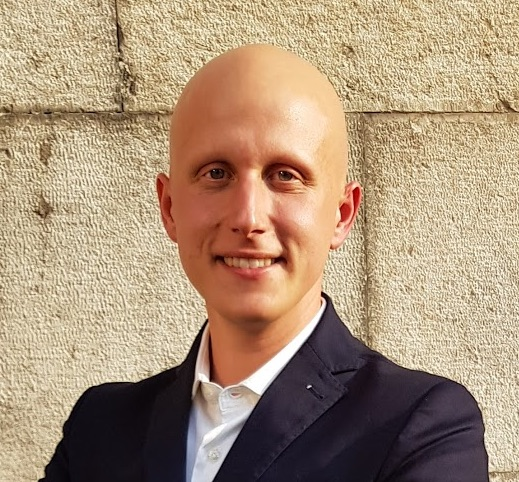
\includegraphics[width=0.8\columnwidth]{matteofico.jpg}\\[\baselineskip] % Your photo
\small % Smaller font size
Matteo Fico \\ % Your name
\url{ficomatteo@gmail.com} \\ % Your email address
\url{linkedin.com/in/matteofico} \\ % Your URL
+39 338 5801268 \\ % Your phone number
\Sep % Some whitespace
\textbf{Address} \\
Via E.Fermi 51 \\ % Address 1
41124, Modena \\ % Address 2
Italy \\ % Address 3
\vfill % Whitespace under this block to push it up under the photo
\end{flushright}
}

%----------------------------------------------------------------------------------------

\begin{document}

\userinformation % Print your information in the left column

\framebreak % End of the first column

%----------------------------------------------------------------------------------------
%	HEADING
%----------------------------------------------------------------------------------------

\cvheading{Matteo Fico} % Large heading - your name

\cvsubheading{Software Engineer} % Subheading - your occupation/specialization

%----------------------------------------------------------------------------------------
%	ABOUT ME
%----------------------------------------------------------------------------------------

\aboutme{About Me}{
	I'm an hardworking and ambitious person who likes to organize his work and optimize it day after day. 
	
	My focus has always been doing my job the best way possible and also take care of communication, especially when you're part of a team.
						
	I think of myself as a thoughtful and logical person and I'd like to improve my communication and management skills.	
	   }
\Sep

%----------------------------------------------------------------------------------------
%	EDUCATION
%----------------------------------------------------------------------------------------

\CVSection{Education}

%------------------------------------------------

\CVItem{July 2013, Unimore, \textit{Università di Modena e Reggio Emilia}}{Bachelor Degree in  Computer Engineering}

%------------------------------------------------

\CVItem{June 2005, ITC Barozzi, \textit{Technical high school}}{Diploma in accounting,business and programming}

%------------------------------------------------

\Sep % Extra whitespace after the end of a major section

%----------------------------------------------------------------------------------------
%	EXPERIENCE
%----------------------------------------------------------------------------------------

\CVSection{Experience}

%------------------------------------------------

\CVItem{Nov 2016 - present, \textit{R\&D Computer Vision Tech}, Unisorting}{
\begin{itemize}
	\item Work on the field:
	\begin{itemize}
		\item Collecting data on the field (images, settings, customer preferences, ...)
		\item Training customer's techs
		\item Tuning computer vision software and hardware
		\item Helping salesmen with demos
		\item Machine supervisory
	\end{itemize}
	\item Office work:
	\begin{itemize}
		\item Tuning software on clients purposes
		\item Tech support on computer vision machine issues
		\item Data Analysis and feasibility study on collected data
		\begin{itemize}
			\item Data analysis with Python and Excel
		\end{itemize}
	\end{itemize}
		\item Software development:
		\begin{itemize} 
		\item C\# side project for data collection 
		\item Python side project for data analysis
		\end{itemize}
\end{itemize}
}

%------------------------------------------------

\CVItem{Aug 2013 - Nov 2016, \textit{Software Developer}, Datagraph S.r.l.}{Main developer on public accounting softwares:
\begin{itemize}
	\item Analysis, development and software management
	\item MS SQL Server maintenance
	\item Customers support and help
\end{itemize}}

\CVItem{Sep 2012 - Aug 2013, \textit{Software technician}, Spin S.r.l.}{ 
\begin{itemize}
	\item Graduation thesis|"Interfacciamento di un sistema di pesatura ed etichettatura"
	\item HMI for Supervisory Control and Data Acquisition.
\end{itemize}}


%----------------------------------------------------------------------------------------
%	NEW PAGE DELIMITER
%	Place this block wherever you would like the content of your CV to go onto the next page
%----------------------------------------------------------------------------------------

\clearpage % Start a new page

\userinformation % Print your information in the left column

\framebreak % End of the first column

\Sep % Extra whitespace after the end of a major section

%----------------------------------------------------------------------------------------
%	IT SKILLS
%----------------------------------------------------------------------------------------

\CVSection{IT Skills}

%------------------------------------------------

\CVItem{Programming}
{C\#, Python, C++}

%------------------------------------------------

\CVItem{DBMS}
{MS SQL, MySQL}

%------------------------------------------------

\CVItem{Web}
{HTML, CSS}

%------------------------------------------------

\CVItem{Source Control}
{Mercurial, GIT, SVN}

%------------------------------------------------

\CVItem{OS}
{Windows, Mac Os X, Unix/Linux}

%----------------------------------------------------------------------------------------
%	PERSONAL SKILLS
%----------------------------------------------------------------------------------------

\Sep % Extra whitespace after the end of a major section

\CVSection{Personal Skills}

\CVItem{Problem-solving and decision-making}{Both improved working on the field}

\CVItem{Team-work}{Enhanced working on complex projects}

\CVItem{Adaptability}{Observation and willingness to learn help me adapting}

\CVItem{Punctuality}{Being punctual shows your respect for others}

\CVItem{Creativity}{Creative approach to problem solving}

%------------------------------------------------

\Sep % Extra whitespace after the end of a major section

\CVSection{Languages}

%------------------------------------------------

\CVItem{Italian}{Native} 

\CVItem{English}{Professional working}

\CVItem{Spanish}{Professional working}

\CVItem{French}{Elementary}

\Sep

%----------------------------------------------------------------------------------------
%	INTERESTS
%----------------------------------------------------------------------------------------

\CVSection{Interests}

%------------------------------------------------

\CVItem{Professional}{Data Analysis, Software Management, UX/UI, Machine Learning}

\CVItem{Personal}{Photography, travel, music, cooking, hiking}

%------------------------------------------------

\Sep % Extra whitespace after the end of a major section

%----------------------------------------------------------------------------------------


\end{document}


